\documentclass[landscape,letterpaper]{article}
\usepackage[left=5pt,top=5pt,right=20pt]{geometry}
\usepackage{tikz}
\begin{document}

\begin{center}
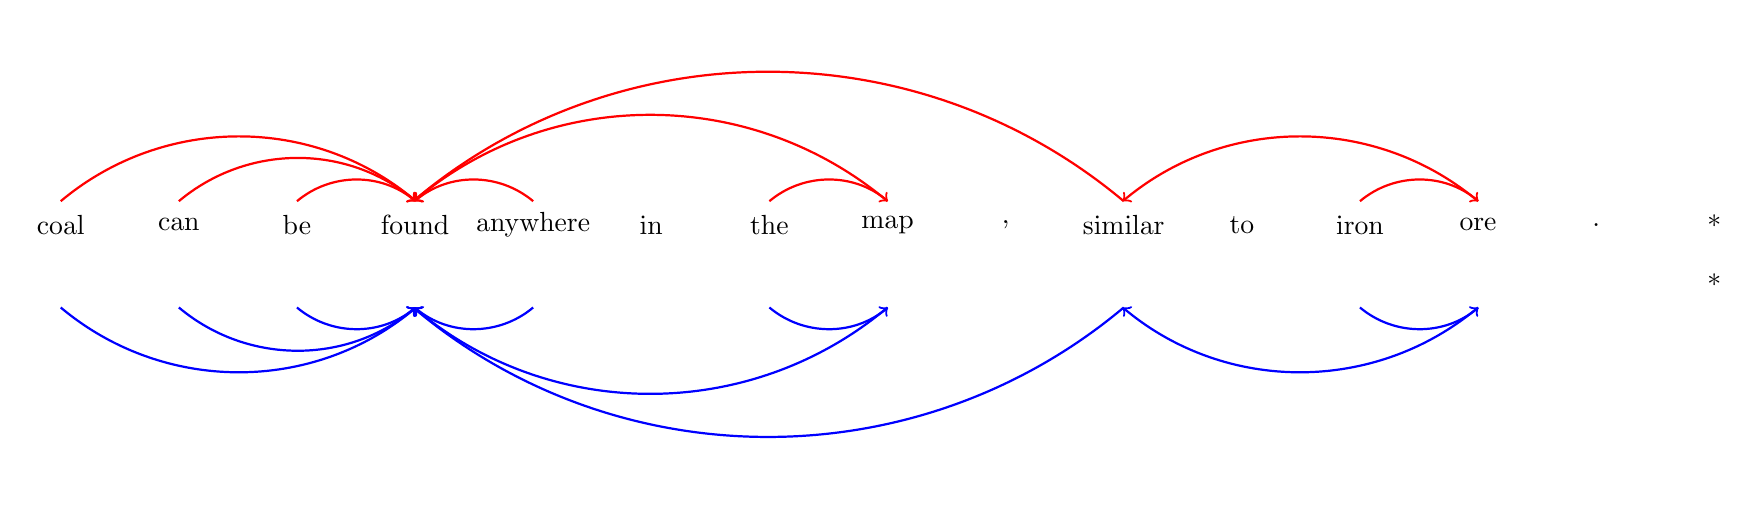
\begin{tikzpicture}[scale=1.5]
\draw(0,0) node {coal};
\draw(0,-0.5) node {};
\draw(1,0) node {can};
\draw(1,-0.5) node {};
\draw(2,0) node {be};
\draw(2,-0.5) node {};
\draw(3,0) node {found};
\draw(3,-0.5) node {};
\draw(4,0) node {anywhere};
\draw(4,-0.5) node {};
\draw(5,0) node {in};
\draw(5,-0.5) node {};
\draw(6,0) node {the};
\draw(6,-0.5) node {};
\draw(7,0) node {map};
\draw(7,-0.5) node {};
\draw(8,0) node {,};
\draw(8,-0.5) node {};
\draw(9,0) node {similar};
\draw(9,-0.5) node {};
\draw(10,0) node {to};
\draw(10,-0.5) node {};
\draw(11,0) node {iron};
\draw(11,-0.5) node {};
\draw(12,0) node {ore};
\draw(12,-0.5) node {};
\draw(13,0) node {.};
\draw(13,-0.5) node {};
\draw(14,0) node {*};
\draw(14,-0.5) node {*};
\draw[thick,red,->] (0,0.2) arc(130:50:2.34);
\draw[thick,red,->] (1,0.2) arc(130:50:1.56);
\draw[thick,red,->] (2,0.2) arc(130:50:0.78);
\draw[thick,red,->] (4,0.2) arc(50:130:0.78);
\draw[thick,red,->] (6,0.2) arc(130:50:0.78);
\draw[thick,red,->] (7,0.2) arc(50:130:3.12);
\draw[thick,red,->] (9,0.2) arc(50:130:4.68);
\draw[thick,red,->] (11,0.2) arc(130:50:0.78);
\draw[thick,red,->] (12,0.2) arc(50:130:2.34);
\draw[thick,blue,->] (0,-0.7) arc(50:130:-2.34);
\draw[thick,blue,->] (1,-0.7) arc(50:130:-1.56);
\draw[thick,blue,->] (2,-0.7) arc(50:130:-0.78);
\draw[thick,blue,->] (4,-0.7) arc(130:50:-0.78);
\draw[thick,blue,->] (6,-0.7) arc(50:130:-0.78);
\draw[thick,blue,->] (7,-0.7) arc(130:50:-3.12);
\draw[thick,blue,->] (9,-0.7) arc(130:50:-4.68);
\draw[thick,blue,->] (11,-0.7) arc(50:130:-0.78);
\draw[thick,blue,->] (12,-0.7) arc(130:50:-2.34);
\end{tikzpicture}
\end{center}

\end{document}